\documentclass[11pt,reqno]{amsart}

\usepackage[utf8]{inputenc}
\usepackage[T1]{fontenc}
\usepackage{amsmath,amssymb,amsthm,mathtools}
\usepackage{booktabs}
\usepackage{graphicx}
\usepackage{geometry}
\usepackage{xcolor}
\usepackage[colorlinks=true,linkcolor=blue!60!black,citecolor=blue!60!black,urlcolor=blue!60!black]{hyperref}

\geometry{margin=1in}
\setlength{\emergencystretch}{3em}

\newtheorem{theorem}{Theorem}[section]
\newtheorem{proposition}[theorem]{Proposition}
\newtheorem{lemma}[theorem]{Lemma}
\newtheorem{corollary}[theorem]{Corollary}
\theoremstyle{definition}
\newtheorem{definition}[theorem]{Definition}
\newtheorem{remark}[theorem]{Remark}

\newcommand{\C}{\mathbb{C}}
\newcommand{\R}{\mathbb{R}}
\newcommand{\Q}{\mathbb{Q}}
\newcommand{\Z}{\mathbb{Z}}
\newcommand{\N}{\mathbb{N}}
\newcommand{\D}{\mathbb{D}}
\newcommand{\T}{\mathbb{T}}
\newcommand{\E}{\mathbb{E}}
\newcommand{\Hilb}{\mathcal{H}}
\newcommand{\KGC}{K_G^{\C}}
\newcommand{\KGR}{K_G^{\R}}
\newcommand{\gd}{\gamma^\dagger}
\newcommand{\ph}{\operatorname{ph}}
\DeclareMathOperator{\RePart}{Re}
\DeclareMathOperator{\ImPart}{Im}

\title[Haagerup's value is a strict upper bound for \texorpdfstring{$\KGC$}{KGC}]{Haagerup's Value Is a Strict Upper Bound for the Complex Grothendieck Constant}
\author{Alin Galatan}
\date{November 2026}

\begin{document}

\begin{abstract}
Let $\KGC$ denote the complex Grothendieck constant. In 1987, Haagerup proved the upper bound $\KGC \le 1/\gamma_H \approx 1.40490913$ via plain complex Gaussian phase rounding and identified the alternating hypergeometric integral
\[
  \begin{gathered}
  \gd \;=\; \int_0^{\pi/2} \frac{\cos^2 t}{\sqrt{1 + \sin^2 t}}\,dt
  \;=\; \frac{\pi}{4}\,{}_2F_1\!\left(\tfrac{1}{2},\tfrac{1}{2};2;-1\right)
  \;=\; 0.711958659778\ldots,\\
  \frac{1}{\gd} \;=\; 1.404575934663\ldots,
  \end{gathered}
\]
whose reciprocal he called ``a perhaps more plausible candidate'' for $\KGC$. We prove that $\KGC$ is strictly below Haagerup's value:
\[
  \KGC \;\le\; \frac{140457588}{10^8} \;=\; 1.40457588 \;<\; \frac{1}{\gd},
\]
thus resolving this conjecture of Haagerup. The bound $1.40457588$ is frozen for this article so that the construction and its formal verification remain as clean and compact as possible; sharper bounds evolve continuously in \url{https://github.com/agalatan/grothendieck-lean}.
Interpreting $1/\KGC$ as the value of a zero-sum game between randomized Gaussian rounders and adversarial Hermite--Wick chaos projections, we show that the alternating adversary $q_k = (-1)^k$ imposes a universal ceiling $W(h) = \sum_{k=0}^\infty (-1)^k h_k$ blocking all convex combinations of preprocessed scalar phase rounders ($|W| \le \gd$) and symmetric smoothed cell rounders on $\C^2$ ($W \approx 0.711920 < \gd$). We cross this barrier with a six-channel rational convex mixture built from two $64 \times 64 \times 36$ Fourier-cell maps on $\C^2$: a reflected pair $(f_{\mathrm{tig}}, g_{\mathrm{tig}})$ with $g_{\mathrm{tig}}(z_1,z_2) = f_{\mathrm{tig}}(-z_1,z_2)$ whose alternating value lifts strictly above $\gd$ ($W \approx 0.712902$), and a rotated Ornstein--Uhlenbeck smoothed map $f_{\mathrm{sm}}$ whose alternating polynomial preprocessors cancel nonlinear chaos distortion across $1 \le k \le 250$ at zero loss in $W$, supplemented by a scalar phase fine-tuning channel. Although none of the six channels beats Haagerup's 1987 bound on its own, destructive interference of their higher harmonics reduces the combined $\ell^1$ distortion below $6.21 \times 10^{-6}$. The ancillary directory \texttt{anc/} is a standalone, hypothesis-free Lean~4 proof of the entire theorem (Appendices~\ref{app:arb} and~\ref{app:lean}). The construction was discovered with AI at the end of a two-month research and formalisation project (Section~\ref{sec:found}).
\end{abstract}

\maketitle

\section{Introduction}

Grothendieck's fundamental inequality \cite{Gro53} asserts the existence of a universal constant $K_G^{\mathbb{F}} < \infty$ over $\mathbb{F} \in \{\R, \C\}$ such that for every finite matrix $A = (A_{pq}) \in \mathbb{F}^{m \times n}$ and every family of vectors $u_1,\dots,u_m, v_1,\dots,v_n$ in the closed unit ball of a Hilbert space $\Hilb$ over $\mathbb{F}$,
\begin{equation}\label{eq:groth-def}
  V(A) \;:=\; \sup_{\|u_p\|_\Hilb \le 1,\, \|v_q\|_\Hilb \le 1}
  \left| \sum_{p=1}^m \sum_{q=1}^n A_{pq} \langle u_p, v_q \rangle_\Hilb \right|
  \;\le\; K_G^{\mathbb{F}} \, C(A),
\end{equation}
where
\[
  C(A) \;:=\; \sup_{|z_p| \le 1,\, |w_q| \le 1} \left|\sum_{p=1}^m \sum_{q=1}^n A_{pq} \bar{z}_p w_q\right|
\]
denotes the classical $\ell^\infty \to \ell^1$ bilinear norm, attained at unimodular scalars $|z_p| = |w_q| = 1$ by convexity; the sharp constant $K_G^{\mathbb{F}}$ is the infimum of all admissible factors in \eqref{eq:groth-def} \cite{Pis12}. Over $\R$, Krivine \cite{Kri79} proved $\KGR \le \pi / (2\ln(1 + \sqrt{2})) \approx 1.78221$ in 1979 and conjectured equality; thirty-two years later, Braverman, Makarychev, Makarychev, and Naor \cite{BMMN11} proved the strict inequality $\KGR < \pi / (2\ln(1 + \sqrt{2}))$ via a two-dimensional Gaussian rounding scheme on $\R^2$.

In the complex case, upper bounds proved considerably more resistant. Improving upon Pisier's complex interpolation bound $\KGC \le e^{1-\gamma} \approx 1.5262$ \cite{Pis78}, Haagerup \cite{Haa87} adapted Krivine's series-reversion method in 1987 to plain complex Gaussian phase rounding $\ph(z) := z/|z|$ ($z \ne 0$, $\ph(0) := 0$) on $\C$. For correlated standard complex Gaussians $(X, Y)$ satisfying $\E[|X|^2] = \E[|Y|^2] = 1$ and $\E[\bar{X} Y] = t \in (-1,1)$, Haagerup derived the Mehler expansion
\begin{equation}\label{eq:phi-haagerup}
  \varphi(t) \;:=\; \E\!\left[\overline{\ph(X)}\,\ph(Y)\right]
  \;=\; \frac{\pi}{4}\, t \, {}_2F_1\!\left(\tfrac{1}{2}, \tfrac{1}{2}; 2; t^2\right)
  \;=\; \sum_{k=0}^\infty r_k \, t^{2k+1},
\end{equation}
where $r_0 = \frac{\pi}{4}$ and $r_{k+1}/r_k = \frac{(2k+1)^2}{4(k+1)(k+2)}$ for $k \ge 0$. Because the reverted series $\varphi^{-1}(u) = \sum_{k=0}^\infty b_k u^{2k+1}$ fails to alternate in sign beyond degree~$5$ ($b_k < 0$ for $k \ge 3$), solving $\sum_{k=0}^\infty |b_k| c^{2k+1} = 1$ yields Haagerup's proved 1987 bound $\KGC \le 1/\gamma_H = 1.4049091327\ldots$ ($\gamma_H = 0.7117898067\ldots$), which stood unimproved for 39 years. Evaluating the alternating series $|\varphi(i)| = \sum_{k=0}^\infty (-1)^k r_k$ directly instead gives Haagerup's alternating integral
\begin{equation}\label{eq:gd-def}
  \begin{gathered}
  \gd \;:=\; \sum_{k=0}^\infty (-1)^k r_k
  \;=\; \int_0^{\pi/2} \frac{\cos^2 t}{\sqrt{1 + \sin^2 t}}\,dt
  \;=\; 0.7119586597782638\ldots,\\
  \frac{1}{\gd} \;=\; 1.4045759346637420\ldots
  \end{gathered}
\end{equation}
Haagerup \cite[p.~202]{Haa87} remarked that his bound $1/\gamma_H$ is probably not sharp and called $1/\gd$ ``a perhaps more plausible candidate'' for $\KGC$.

Very recently, both the real and complex constants saw a wave of renewed progress: over $\R$, Saha, Li, Xue, Chaudhuri, Klivans, Kothari, and Meka \cite{SLX26} sharpened the two-chaos Krivine approach via Gaussianized Rademacher chaos, and Heilman, Jones, and Malavolta \cite{HJM26b} combined primal/dual Hermite searches to place $\KGR \in [1.773, 1.7799]$; over $\C$, Heilman, Jones, and Malavolta \cite{HJM26} obtained the first strict improvement below $1/\gamma_H$, proving $\KGC < 1.40489856$ via convex mixtures of preprocessed scalar phase rounders (alongside the lower bound $\KGC > 1.4$, building on Davie \cite{Dav84}, K\"onig \cite{Kon90}, and Guo--Fang--Lu \cite{GFL26}). The Lean~4 development \cite{Gal26} proves, without hypotheses, $1.4018 < \KGC \le 1.40457588$. Its upper bound comes from a six-channel mixture of the same kind as the one here, with every channel estimate checked in Lean, and is therefore itself below $1/\gd$ (Appendix~\ref{app:lean}).

In this paper we cross Haagerup's barrier $1/\gd$: his value is a strict upper bound for $\KGC$.

\begin{theorem}[Main Result]\label{thm:main}
The complex Grothendieck constant satisfies
\[
  \KGC \;\le\; \frac{140457588}{10^8}
  \;=\; 1.40457588
  \;<\; \frac{1}{\gd}
  \;=\; 1.404575934663\ldots
\]
In particular, Haagerup's value $1/\gd$ is a strict upper bound for $\KGC$.
\end{theorem}

The rational bound $\frac{140457588}{10^8}$ in Theorem~\ref{thm:main} is proved without hypotheses in the standalone Lean~4 package in \texttt{anc/} (Appendices~\ref{app:arb} and~\ref{app:lean}), frozen at this value to keep the certificate self-contained and compact while sharper bounds ($1.4018 < \KGC \le 1.40457588$ at the time of writing) continue to evolve in \cite{Gal26}.

Theorem~\ref{thm:main} is the complex counterpart of the theorem of Braverman, Makarychev, Makarychev, and Naor \cite{BMMN11} that Krivine's bound is not sharp, but the geometry of the barrier is markedly different. Over $\R$, Krivine's constant is already achieved by a single 1D sign rounder whose inverse series alternates cleanly. Over $\C$, 1D phase mixtures saturate near $1.404898$ \cite{HJM26}, well above $1/\gd$, and even passing to symmetric $\C^2$ rounders leaves $\gd$ untouched: as shown in Section~\ref{sec:obstruction}, $\gd$ is enforced by an alternating Hermite adversary that blocks every convex combination of preprocessed scalar phase channels and our symmetric smoothed cell rounders on $\C^2$. Crossing $\gd$ requires breaking row--column symmetry on $\C^2$ via the reflection $(z_1, z_2) \mapsto (-z_1, z_2)$ and pairing that reflected channel with symmetric steering channels in a six-strategy mixture.

\section{Rounding, Hermite Games, and Why Mixtures Win}\label{sec:obstruction}

Before introducing the two-coordinate cell maps of Section~\ref{sec:mechanism}, it is worth stepping back to ask what every upper-bound construction since Grothendieck \cite{Gro53} is actually optimizing, who the implicit adversary is, and why modern bounds invariably rely on convex mixtures (``soups'') of several rounding strategies rather than a single polished map.

\subsection{Primal Radial Transfer and the Hunt for Pure Linearity}
We take inner products $\langle u, v \rangle_\Hilb$ to be conjugate-linear in the first slot and linear in the second. Because every matrix $A \in \C^{m \times n}$ acts on the finite-dimensional span of $\{u_1,\dots,u_m, v_1,\dots,v_n\}$, it suffices in \eqref{eq:groth-def} to range over $\Hilb = \C^N$ ($N \ge 1$) with $\langle u, v \rangle = \sum_{r=1}^N \bar{u}_r v_r$.

Every Gaussian rounding scheme converts Hilbert-space inner products $\zeta_{pq} := \langle u_p, v_q \rangle \in \overline{\D}$ into random disk-valued scalars $Z_p, W_q \in \overline{\D}$ whose expected correlation has a radial series expansion
\[
  \E[\bar{Z}_p W_q] \;=\; H(\zeta_{pq}) \;=\; \sum_{k=0}^\infty h_k \, \zeta_{pq} |\zeta_{pq}|^{2k}, \qquad h_k \in \R.
\]
If a rounding scheme could realize a purely linear correlation $H(\zeta) = h_0 \zeta$ with $h_0 > 0$ and $h_k = 0$ for all $k \ge 1$, Jensen's inequality would immediately yield $h_0 V(A) \le C(A)$, hence $\KGC \le 1/h_0$. However, no non-zero linear functional on Gaussian space stays bounded in the unit disk $\overline{\D}$: clamping outputs to $|Z_p|, |W_q| \le 1$ inevitably generates \emph{nonlinear harmonic distortion} across higher odd powers $\zeta |\zeta|^{2k}$ ($k \ge 1$).

From Krivine \cite{Kri79} to the present, every upper-bound proof is a method for cancelling or bounding this higher-order distortion while preserving as much of the linear slope $h_0$ as possible. Krivine \cite{Kri79}, Haagerup \cite{Haa87}, Braverman et al.\ \cite{BMMN11}, and Saha et al.\ \cite{SLX26} cancel $h_k$ ($k \ge 1$) \emph{before} rounding, by lifting $u_p, v_q$ into an infinite direct sum of tensor powers to invert $H$ analytically. Following the primal viewpoint developed in \cite{HJM26,HJM26b,Gal26}, one can bypass series inversion altogether and pay for residual nonlinear harmonics directly in $\ell^1$: as noted in \cite[Lemma~3.5]{HJM26}, the resulting budget $D(h) = h_0 - \sum_{k=1}^\infty |h_k|$ is exact for optimal tensor-power repair.

\begin{lemma}[Radial Schur Transfer]\label{lem:transfer}
Let $h = (h_k)_{k \ge 0}$ be an absolutely summable real sequence such that for every matrix $A \in \C^{m \times n}$ and unit-ball vectors $u_1,\dots,u_m, v_1,\dots,v_n \in \C^N$,
\begin{equation}\label{eq:dominated}
  \left| \sum_{k=0}^\infty h_k \sum_{p=1}^m \sum_{q=1}^n A_{pq} \langle u_p, v_q \rangle \big|\langle u_p, v_q \rangle\big|^{2k} \right|
  \;\le\; C(A).
\end{equation}
If $D(h) := h_0 - \sum_{k=1}^\infty |h_k| > 0$, then $\KGC \le 1 / D(h)$. Moreover, the set $\mathcal{C} \subset \ell^1(\N)$ of real sequences satisfying \eqref{eq:dominated} is convex.
\end{lemma}

\begin{proof}
Fix $N \ge 1$, $A \in \C^{m \times n}$, and unit-ball vectors $u_p, v_q \in \C^N$. For each integer $k \ge 0$ and $x \in \C^N$, consider the mixed tensor vector
\[
  \Psi_k(x) \;:=\; x^{\otimes (k+1)} \otimes \bar{x}^{\otimes k} \;\in\; \C^{N^{2k+1}},
\]
where $\bar{x} = (\bar{x}_1,\dots,\bar{x}_N)$. Multiplicativity of Euclidean inner products under Kronecker products gives $\|\Psi_k(x)\|_2 = \|x\|_2^{2k+1} \le 1$ whenever $\|x\|_2 \le 1$, together with
\[
  \langle \Psi_k(u_p), \Psi_k(v_q) \rangle
  \;=\; \langle u_p, v_q \rangle^{k+1} \overline{\langle u_p, v_q \rangle}^{\,k}
  \;=\; \langle u_p, v_q \rangle \big|\langle u_p, v_q \rangle\big|^{2k}.
\]
Each bilinear form $S_k := \sum_{p,q} A_{pq} \langle u_p, v_q \rangle |\langle u_p, v_q \rangle|^{2k}$ is therefore realized by unit-ball vectors in $\C^{N^{2k+1}}$, whence $|S_k| \le V(A)$ for all $k \ge 0$. By the reverse triangle inequality and \eqref{eq:dominated},
\[
  h_0 |S_0| - \left(\sum_{k=1}^\infty |h_k|\right) V(A)
  \;\le\; |h_0 S_0| - \left|\sum_{k=1}^\infty h_k S_k\right|
  \;\le\; \left|\sum_{k=0}^\infty h_k S_k\right|
  \;\le\; C(A).
\]
Rearranging gives $h_0 |S_0| \le C(A) + \big(\sum_{k=1}^\infty |h_k|\big) V(A)$. Taking the supremum over $N \ge 1$ and $\|u_p\|_2, \|v_q\|_2 \le 1$ yields $D(h) V(A) \le C(A)$. Convexity of $\mathcal{C}$ follows immediately from absolute summability, Fubini summation, and the triangle inequality.
\end{proof}

\subsection{The Adversarial Hermite Game and the Alternating Barrier}
Lemma~\ref{lem:transfer} admits a transparent zero-sum game interpretation, mirroring the Gaussian minimax duality established by Raghavendra--Steurer \cite{RS09}, Naor--Regev \cite{NR14}, and Heilman--Jones--Malavolta \cite{HJM26b}. Notice the identity
\begin{equation}\label{eq:minimax-form}
  D(h) \;=\; h_0 - \sum_{k=1}^\infty |h_k|
  \;=\; \inf_{q_0 = 1,\; |q_k| \le 1} \sum_{k=0}^\infty q_k h_k.
\end{equation}
Here the two players are:
\begin{itemize}
  \item \textbf{The Rounder (upper-bound player):} selects a realizable correlation sequence $h \in \mathcal{C}$ via randomized disk-valued maps on complex Gaussian space, striving to maximize $D(h)$.
  \item \textbf{The Adversary (lower-bound player):} selects a multiplier sequence $q = (1, q_1, q_2, \dots)$ with $q_k \in [-1, 1]$, representing a continuous matrix kernel $Q(z, w) = P_{1,0}(z, w) + \sum_{k=1}^\infty q_k P_{k+1,k}(z, w)$ built from the orthogonal projectors $P_{k+1,k}$ onto the charge-$1$ complex Hermite--Wick chaos subspaces of bidegree $(k+1, k)$ on Gaussian space $(\C^N, \gamma_{\C^N})$ as $N \to \infty$.
\end{itemize}
Why does this adversary have leverage? Coordinate vectors $u_z = z/\sqrt{N}$ live purely in the degree-$1$ linear chaos $P_{1,0}$, where every higher projector $P_{k+1,k}$ ($k \ge 1$) vanishes identically; thus $Q$ retains unit vector value $V \ge 1$. By contrast, any unimodular scalar rounding $|Z(z)| = |W(w)| = 1$ must spill $L^2$-energy into higher chaoses $k \ge 1$, and the adversary chooses $q_k = -\operatorname{sgn}(h_k)$ to penalize every mode in which the rounder leaks correlation. Concrete lower bounds for $\KGC$ are explicit instances of this adversary: Davie \cite{Dav84} and Guo--Fang--Lu \cite{GFL26} penalize all higher modes uniformly ($q_k = -\lambda$), while \cite{HJM26,Gal26} concentrate negative weight on cubic chaos $P_{2,1}$ ($k = 1$).

Comparing $\R$ and $\C$ clarifies why the complex game is subtler. Over $\R$, binary rounders $f, g : \R^d \to \{\pm 1\}$ decompose into $f_+ = \frac{1}{2}(f+g)$ and $f_- = \frac{1}{2}(f-g)$ taking values in $\{-1,0,1\}$ with \emph{disjoint supports} ($f_+ f_- \equiv 0$, \cite[Prop.~2.4]{HJM26b}), decoupling the symmetric and antisymmetric parts of the game, while $\arcsin^{-1}(u) = \sin u$ alternates in sign at every odd degree. Over $\C$, unimodular outputs $e^{i(\alpha+\theta)}$ and $e^{i(\alpha-\theta)}$ remain coupled through a shared continuous phase $\alpha \in \R/2\pi\Z$, and $\varphi^{-1}(u)$ loses sign alternation at degree~$7$.

In the complex game, one specific adversary explains why $1/\gd$ stood as a natural barrier: the \emph{alternating adversary} $q_k = (-1)^k$ (studied in finite dimensions by K\"onig \cite{Kon90}), whose payoff against a rounder $h \in \ell^1(\N)$ is the \emph{alternating ceiling functional}
\[
  W(h) \;:=\; \sum_{k=0}^\infty (-1)^k h_k.
\]

\begin{proposition}[Universal Alternating Ceiling and Convex No-Go]\label{prop:nogo}
For every absolutely summable real sequence $h = (h_k)_{k \ge 0}$, one has
\[
  D(h) \;\le\; W(h) \;\le\; |W(h)|.
\]
Consequently, if $h^{(1)}, \dots, h^{(M)} \in \ell^1(\N)$ satisfy $W(h^{(i)}) \le C$ for all $1 \le i \le M$, then every convex combination $H = \sum_{i=1}^M w_i h^{(i)}$ ($w_i \ge 0$, $\sum_{i=1}^M w_i = 1$) satisfies $D(H) \le C$.
\end{proposition}

\begin{proof}
Setting $q_k = (-1)^k \in \{\pm 1\}$ in \eqref{eq:minimax-form} gives $-(-1)^k h_k \le |h_k|$ for each $k \ge 1$, so $D(h) = h_0 - \sum_{k=1}^\infty |h_k| \le h_0 + \sum_{k=1}^\infty (-1)^k h_k = W(h) \le |W(h)|$. By linearity of $W$, $D(H) \le W(H) = \sum_{i=1}^M w_i W(h^{(i)}) \le C$.
\end{proof}

Proposition~\ref{prop:nogo} pinpoints the exact obstruction faced by scalar phase channels and symmetric $\C^2$ rounders:
\begin{enumerate}
  \item \textbf{Preprocessed scalar phase channels:} Composing plain phase rounding $\ph(z) = z/|z|$ with any contractive odd polynomial preprocessor $\rho(\zeta) = \zeta R(|\zeta|^2)$, where $R(X) = \sum_{j=0}^d a_j X^j \in \R[X]$ satisfies $\|R\|_1 := \sum_j |a_j| \le 1$, produces the radial series $\sum_{k=0}^\infty h_k \zeta |\zeta|^{2k}$ with
  \[
    h_k \;=\; \sum_{m=0}^k r_m\, [X^{k-m}]\, R(X)^{2m+1}.
  \]
  Setting $X = -1$ gives $\sigma := R(-1) \in [-1,1]$ and $W(h) = \sum_{m=0}^\infty (-1)^m r_m \sigma^{2m+1}$. Since $(r_m)_{m \ge 0}$ is strictly positive and strictly decreasing ($r_{m+1}/r_m = \frac{(2m+1)^2}{4(m+1)(m+2)} < 1$), grouping consecutive pairs $(2\ell, 2\ell+1)$ shows $\sum_{m=0}^\infty (-1)^m r_m \tau^{2m+1} \ge 0$ for all $\tau = |\sigma| \in [0,1]$. This sum equals $\tau\int_0^{\pi/2} \cos^2 t\,(1+\tau^2\sin^2 t)^{-1/2}\,dt$, whose derivative in $\tau$ is $\int_0^{\pi/2} \cos^2 t\,(1+\tau^2\sin^2 t)^{-3/2}\,dt > 0$, so it attains its maximum $\gd$ at $\tau = 1$. As $W(h)$ is odd in $\sigma$, $|W(h)| \le \gd$ identically.
  \item \textbf{Symmetric smoothed cell channels on $\C^2$:} Our symmetric smoothed two-coordinate rounder $f_{\mathrm{sm}} : \C^2 \to \overline{\D}$ (Section~\ref{sec:mechanism}), evaluated at its optimal alternating signs $(P(-1), Q(-1)) = (1, 1)$, achieves $W(f_{\mathrm{sm}}) = 0.71191988\ldots < \gd$ ($3.88 \times 10^{-5}$ below $\gd$).
\end{enumerate}
By Proposition~\ref{prop:nogo}, \emph{no} convex combination of preprocessed scalar phase channels and symmetric $f_{\mathrm{sm}}$ channels can ever achieve $D(H) > \gd$. Against those families, the alternating adversary $q_k = (-1)^k$ is unbeatable; crossing $\gd$ requires at least one rounding strategy with $W > \gd$.

\subsection{Why a Convex ``Soup'' of Strategies Wins}
Once one strategy achieves $W > \gd$, why not use it alone instead of mixing six strategies with unequal weights? Three structural principles force a randomized mixture:
\begin{enumerate}
  \item \textbf{Parseval rigidity of pure strategies:} Any single measurable rounder $G : \C^d \to \overline{\D}$ has $\|G\|_{L^2}^2 \le 1$ while its linear projection satisfies $h_0 < 1$; by Parseval's identity, the remaining energy must appear across higher Hermite modes, leaving a fixed sign signature $(h_1, h_2, \dots)$ that the adversary punishes via $q_k = -\operatorname{sgn}(h_k)$.
  \item \textbf{Killing nonlinear correlation while keeping linear correlation:} Tossing a biased die to pick channel $p$ with probability $w_p$ averages the correlation curves $H = \sum_p w_p h^{(p)}$. Because every channel has $h_0^{(p)} > 0$, their linear slopes add \emph{constructively}, whereas channels equipped with different preprocessors carry \emph{opposite signs} on higher modes $k \ge 1$ and interfere \emph{destructively} ($\sum_p w_p h_k^{(p)} \approx 0$). Mixing does not kill correlation indiscriminately: it selectively annihilates higher-order harmonic correlation so the average behaves almost like a pure linear map $H(\zeta) \approx H_0 \zeta$.
  \item \textbf{Division of labor among specialists:} Breaking row--column symmetry on $\C^2$ lifts $W$ comfortably above $\gd$ ($W \approx 0.712902$), defeating the alternating adversary $q_k = (-1)^k$, but creates large non-alternating head residuals ($\sum_{k \ge 1} |h_k| \approx 0.0253$ even after linear preprocessing, giving only $\KGC \le 1.4460$ alone). Conversely, symmetric smoothed $\C^2$ channels have $W < \gd$ (and alone give at best $1.4075$), yet under alternating preprocessors they span rich Hermite decay profiles at \emph{zero loss in $W$}. Weighting the high-ceiling specialist at ${\sim}5.65\%$ and the low-distortion steering workhorses at ${\sim}94.35\%$ captures both advantages simultaneously: none of the six channels in Table~\ref{tab:cert} beats Haagerup's $1.404909$ individually, yet their convex combination proves $\KGC \le 1.40457588 < 1/\gd$.
\end{enumerate}

\section{Two-Coordinate Cell Rounders, Reflection, and Steering}\label{sec:mechanism}

\subsection{Unified Holomorphic Gaussian Realization on \texorpdfstring{$\C^2$}{C2}}
Every channel in our certificate is an instance of a single Gaussian realization mechanism on $\C^2$. Let $\gamma_{\C}(dz) = \pi^{-1} e^{-|z|^2}\,dA(z)$ denote the standard complex Gaussian measure on $\C$, with product measure $\gamma_{\C^2} = \gamma_{\C} \otimes \gamma_{\C}$ on $\C^2$. Let $G : \C^2 \to \overline{\D}$ be a measurable map satisfying diagonal $U(1)$-equivariance (charge~$1$),
\begin{equation}\label{eq:charge-one}
  G(c z_1, c z_2) \;=\; c\, G(z_1, z_2) \qquad \text{for all } c \in \C \text{ with } |c| = 1 \text{ and } (z_1, z_2) \in \C^2.
\end{equation}
Fix two real polynomials $P(X) = \sum_{j=0}^{M_1} p_j X^j$ and $Q(X) = \sum_{j=0}^{M_2} q_j X^j$ satisfying $\|P\|_1 \le 1$ and $\|Q\|_1 \le 1$. Given unit-ball vectors $u_p, v_q \in \C^N$ with $\zeta_{pq} := \langle u_p, v_q \rangle \in \overline{\D}$, set
\[
  \rho_1(\zeta) \;:=\; \zeta P(|\zeta|^2), \qquad \rho_2(\zeta) \;:=\; \zeta Q(|\zeta|^2).
\]
Form the orthogonal direct sum of scaled mixed tensor lifts $\sqrt{|p_j|}\,\Psi_j(u_p)$ and $\operatorname{sgn}(p_j)\sqrt{|p_j|}\,\Psi_j(v_q)$ (padded by orthogonal slack coordinates so every lifted vector has unit norm, since $\|u_p\|_2, \|v_q\|_2 \le 1$ and $\|P\|_1 \le 1$), and independently do the same for $Q$. Contracting the two lifted spaces against independent standard complex Gaussian vectors produces centered complex Gaussian pairs $X_p = (X_{p,1}, X_{p,2}) \sim \gamma_{\C^2}$ and $Y_q = (Y_{q,1}, Y_{q,2}) \sim \gamma_{\C^2}$ with independent coordinates and holomorphic cross-correlations
\[
  \E\!\left[\bar{X}_{p,1} Y_{q,1}\right] \;=\; \rho_1(\zeta_{pq}),
  \qquad
  \E\!\left[\bar{X}_{p,2} Y_{q,2}\right] \;=\; \rho_2(\zeta_{pq}).
\]
Since $|G(X_p)| \le 1$ and $|G(Y_q)| \le 1$ pointwise on every sample realization, Jensen's inequality gives
\[
  \left|\sum_{p,q} A_{pq} \, \E\!\left[\overline{G(X_p)}\, G(Y_q)\right]\right|
  \;\le\; \E\!\left[\left|\sum_{p,q} A_{pq} \, \overline{G(X_p)}\, G(Y_q)\right|\right]
  \;\le\; C(A).
\]
To read off the radial Taylor expansion of $\E[\overline{G(X_p)}\, G(Y_q)]$, let $\{h_{a,b}\}_{a,b \ge 0}$ denote the orthonormal complex Hermite--Wick basis of $L^2(\C, \gamma_{\C})$, under which Mehler's formula diagonalizes correlation: $\E[\overline{h_{a,b}(X)} h_{a',b'}(Y)] = \delta_{a,a'}\delta_{b,b'} \rho^a \bar{\rho}^b$ whenever $\E[\bar{X} Y] = \rho \in \overline{\D}$. By \eqref{eq:charge-one}, $G$ is supported on tensor basis elements $h_{p_1,q_1}(z_1) h_{p_2,q_2}(z_2)$ of total charge $(p_1 - q_1) + (p_2 - q_2) = 1$, for which $d_1 + d_2$ is odd ($d_r := p_r + q_r$) and
\[
  \rho_1^{p_1}\bar{\rho}_1^{q_1} \rho_2^{p_2}\bar{\rho}_2^{q_2}
  \;=\; \zeta\, |\zeta|^{2(\lfloor d_1/2\rfloor + \lfloor d_2/2\rfloor)} P(|\zeta|^2)^{d_1} Q(|\zeta|^2)^{d_2}.
\]
Grouping basis elements by total coordinate degrees $(d_1, d_2)$ defines the non-negative \emph{bivariate Hermite energy}
\[
  E_G(d_1, d_2) \;:=\; \sum_{\substack{p_1 + q_1 = d_1,\; p_2 + q_2 = d_2 \\ (p_1 - q_1) + (p_2 - q_2) = 1}}
  \big|\langle h_{p_1,q_1} \otimes h_{p_2,q_2},\, G \rangle_{L^2(\gamma_{\C^2})}\big|^2 \;\ge\; 0,
\]
with $\sum_{d_1, d_2} E_G(d_1, d_2) = \|G\|_{L^2(\gamma_{\C^2})}^2 \le 1$, and yields the exact dominated radial series $\sum_{k=0}^\infty h_k \zeta_{pq} |\zeta_{pq}|^{2k}$ with automatically real coefficients
\begin{equation}\label{eq:bivar-kernel}
  h_k \;=\; \sum_{d_1 + d_2 \text{ odd}} E_G(d_1, d_2) \, [X^k]\!\left(X^{\lfloor d_1/2 \rfloor + \lfloor d_2/2 \rfloor} P(X)^{d_1} Q(X)^{d_2}\right).
\end{equation}
Notice that when $G(z_1, z_2) = \ph(z_1)$ depends only on the first coordinate and $Q \equiv 0$, $E_G(2m+1, 0) = r_m$ and \eqref{eq:bivar-kernel} reduces immediately to Haagerup's preprocessed scalar series $h_k = \sum_{m=0}^k r_m [X^{k-m}] P(X)^{2m+1}$.

\subsection{Parametric \texorpdfstring{$64 \times 64 \times 36$}{64 x 64 x 36} Fourier-Cell Maps and Fej\'er--Riesz Certificates}
Both of our two-coordinate maps belong to a single piecewise-trigonometric family on $\C^2$. Partition $[0, 6)^2$ into $64 \times 64 = 4{,}096$ radial squares $I_i \times I_j$ of width $\frac{3}{32}$, where $I_i := [\frac{3i}{32}, \frac{3(i+1)}{32})$ ($0 \le i < 64$). Given integer tables $c_{r,\ell,i,j}, c_{i,\ell,i,j} \in \Z$ ($0 \le \ell < 36$), set $F(z_1, z_2) := 0$ if $z_1 = 0$, $z_2 = 0$, $|z_1| \ge 6$, or $|z_2| \ge 6$, and otherwise set
\begin{equation}\label{eq:cell-fn}
  F(z_1, z_2) \;:=\; \ph(z_2)\, \bar{w}^{17} \sum_{\ell=0}^{35} \frac{c_{r,\ell,i,j} + i\, c_{i,\ell,i,j}}{2^{24}}\, w^\ell,
  \qquad w \;:=\; \ph(z_1)\,\overline{\ph(z_2)} \;\in\; \T,
\end{equation}
for $(|z_1|, |z_2|) \in I_i \times I_j$. Since $\ph(c z_r) = c\,\ph(z_r)$ leaves $w$ and $(|z_1|, |z_2|)$ invariant when $|c| = 1$, $F$ satisfies \eqref{eq:charge-one}, and writing $m = \ell - 17 \in [-17, 18]$ expands $F$ on each cell into $36$ exact relative-phase harmonics $\ph(z_2) w^m = e^{i m \theta_1 + i(1-m)\theta_2}$.

Certifying $|F(z_1, z_2)| \le 1$ uniformly over the continuous circle $w \in \T$ on all $4{,}096$ cells requires no calculus or grid sampling: each cell carries a companion integer Fej\'er--Riesz polynomial $Q_{i,j}(w) = \sum_{\ell=0}^{35} (q_{r,\ell,i,j} + i\, q_{i,\ell,i,j}) w^\ell$ chosen so that $1 - 2^{-48}|C_{i,j}(w)|^2 \approx 2^{-48}|Q_{i,j}(w)|^2$. Expanding $|C_{i,j}(w)|^2 + |Q_{i,j}(w)|^2 = \sum_{m=-35}^{35} D_m w^m$ on $|w| = 1$, where $D_m = \sum_{d=0}^{35-m} (C_{d+m}\bar{C}_d + Q_{d+m}\bar{Q}_d)$ for $m \ge 0$, every off-diagonal autocorrelation $D_m$ ($m \ge 1$) cancels down to rounding noise, and the triangle inequality gives the exact integer bound
\[
  \big|C_{i,j}(w)\big|^2 \;\le\; \big|C_{i,j}(w)\big|^2 + \big|Q_{i,j}(w)\big|^2
  \;\le\; D_0 + 2 \sum_{m=1}^{35} \big(|\RePart D_m| + |\ImPart D_m|\big) \;\le\; 2^{48},
\]
whence $|F(z_1, z_2)| = 2^{-24}|C_{i,j}(w)| \le 1$ everywhere on $\C^2$.

\subsection{Antisymmetric Reflection on \texorpdfstring{$f_{\mathrm{tig}}$}{f\_tig} (\texorpdfstring{$W > \gd$}{W > gamma-dagger})}
Choose $G = f_{\mathrm{tig}}$ from the $64 \times 64 \times 36$ cell family \eqref{eq:cell-fn} and couple the two coordinates antisymmetrically via $(P, Q) = (-R, +R)$ for a contractive polynomial $R(X)$. Under $(\rho_1, \rho_2) = (-\zeta R(|\zeta|^2), +\zeta R(|\zeta|^2))$, negating $X_{p,1} \mapsto -X_{p,1}$ preserves the law $\gamma_{\C^2}$ while turning the cross-correlations into $(+\zeta R(|\zeta|^2), +\zeta R(|\zeta|^2))$ for the reflected pair
\[
  f_{\mathrm{tig}}(z_1, z_2), \qquad g_{\mathrm{tig}}(z_1, z_2) \;:=\; f_{\mathrm{tig}}(-z_1, z_2).
\]
Accordingly, in \eqref{eq:bivar-kernel} the bivariate series collapses to a 1D convolution: since $(-R(X))^{d_1} R(X)^{d_2} = (-1)^{d_1} R(X)^{2n+1}$ whenever $d_1 + d_2 = 2n + 1$, we obtain
\[
  h_k \;=\; \sum_{n=0}^k \mu_n(f_{\mathrm{tig}})\, [X^{k-n}]\, R(X)^{2n+1},
  \qquad
  \mu_n(f_{\mathrm{tig}}) \;:=\; \sum_{d_1 + d_2 = 2n + 1} (-1)^{d_1} E_{f_{\mathrm{tig}}}(d_1, d_2).
\]
In polar coordinates $z_r = |z_r| e^{i\theta_r}$, let $\phi_{n,a}(s) := \sqrt{\frac{n!}{(n+a)!}}\, s^{a/2} L_n^{(a)}(s)$ ($s = |z|^2$) denote the orthonormal generalized Laguerre basis of $L^2((0,\infty), e^{-s}ds)$. Each angular harmonic $m = \ell - 17 \in [-17, 18]$ has minimum radial index $k_0(m) := (|m| + |1-m| - 1)/2$ and parity $(-1)^{d_1} = (-1)^m$, giving the exact $36$-mode sum
\begin{equation}\label{eq:mu-tiger}
  \mu_n(f_{\mathrm{tig}}) \;=\; \sum_{m = -17}^{18} (-1)^m \sum_{k_0(m) + n_1 + n_2 = n}
  \left|\sum_{i,j=0}^{63} \frac{c_{r,m+17,i,j} + i\,c_{i,m+17,i,j}}{2^{24}}\, J_{n_1,|m|,i}\, J_{n_2,|1-m|,j}\right|^2,
\end{equation}
where $J_{n,a,i} := \int_{9i^2/1024}^{9(i+1)^2/1024} \phi_{n,a}(s) e^{-s}\,ds$ (with zero omitted angular modes, since $f_{\mathrm{tig}}$ has finite Fourier support $m \in [-17, 18]$).

\begin{figure}[htbp]
  \centering
  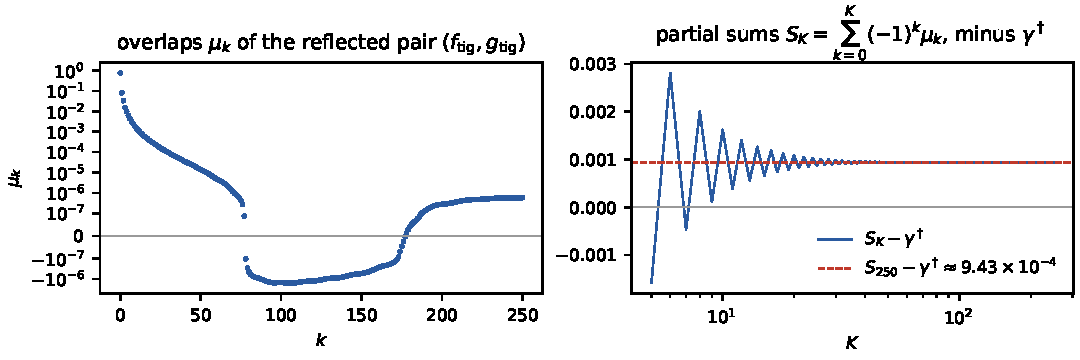
\includegraphics[width=0.95\textwidth]{figures/tiger_mu.pdf}
  \caption{Left: certified radial overlaps $\mu_k(f_{\mathrm{tig}})$ ($0 \le k \le 250$) of the reflected $64 \times 64 \times 36$ cell pair $(f_{\mathrm{tig}}, g_{\mathrm{tig}})$. Right: alternating partial sums $S_K = \sum_{k=0}^K (-1)^k \mu_k(f_{\mathrm{tig}})$ minus Haagerup's constant $\gd$, converging to $+9.43 \times 10^{-4}$ above $\gd$.}\label{fig:tiger-mu}
\end{figure}

Look at the sign in $W(f_{\mathrm{tig}}) = \sum_{n=0}^\infty (-1)^n \mu_n(f_{\mathrm{tig}})$: for any symmetric scheme $(Q = +P)$, cubic modes ($n = 1$) enter $W$ with weight $(-1)^1 \le 0$. Under reflection $z_1 \mapsto -z_1$, odd angular harmonics ($m = 1$, where $k_0(1) = 0$) carry $(-1)^m = -1$, so at $n = 1$ ($n_1 + n_2 = 1$, such as the mixed cubic chaos $z_1(|z_2|^2 - 1)$) the product $(-1)^n (-1)^m = +1$ turns \emph{positive}, destabilizing the plain phase saddle upward. Optimizing the $64 \times 64 \times 36$ Fourier table yields (Figure~\ref{fig:tiger-mu})
\[
  W_{250}(f_{\mathrm{tig}}) \;=\; \sum_{n=0}^{250} (-1)^n \mu_n(f_{\mathrm{tig}}) \;=\; 0.71290157\ldots \;>\; \gd + 9.429 \times 10^{-4}.
\]
Composing $f_{\mathrm{tig}}$ with a two-term alternating linear polynomial $R(X) = c_0 - c_1 X$ ($c_0, c_1 > 0$, $c_0 + c_1 = 1$, Channels~$3$ and~$4$ of Table~\ref{tab:cert}) satisfies $R(-1) = c_0 + c_1 = 1$---preserving $100\%$ of the alternating lift $W > \gd$---while contracting $|R(1)| = c_0 - c_1 < 1$ on the unit circle so that the correlation kernel extends holomorphically beyond $|t| = 1$ with rapidly decaying Hardy tail.

\subsection{Rotated Ornstein--Uhlenbeck Smoothing and Zero-Cost Residual Steering}
Used on its own, $f_{\mathrm{tig}}$ has $\sum_{n=1}^{250} |\mu_n(f_{\mathrm{tig}})| \approx 0.16923$ ($1/D_{250} \approx 1.6641$). To cancel its non-alternating head modes without eroding the linear slope, we pair it with a smoothed symmetric rounder $f_{\mathrm{sm}} : \C^2 \to \overline{\D}$ built from our second $64 \times 64 \times 36$ cell map $T_{\mathrm{cell}}$ via rotated Ornstein--Uhlenbeck smoothing:
\begin{equation}\label{eq:smooth-map}
  f_{\mathrm{sm}}(z_1, z_2) \;:=\; \int_{\C} T_{\mathrm{cell}}\!\Big(c_\theta z_1 + s_\theta z_2,\; s_\eta(-s_\theta z_1 + c_\theta z_2) + c_\eta \xi\Big)\, d\gamma_{\C}(\xi),
\end{equation}
at the exact Pythagorean rational pairs
\[
  (c_\theta, s_\theta) \;=\; \left(\frac{23187}{24245},\, \frac{7084}{24245}\right),
  \qquad
  (s_\eta, c_\eta) \;=\; \left(\frac{87841}{98209},\, \frac{43920}{98209}\right),
\]
satisfying $c_\theta^2 + s_\theta^2 = 1$ and $s_\eta^2 + c_\eta^2 = 1$. Averaging against $\gamma_{\C}$ preserves measurability, $|f_{\mathrm{sm}}| \le 1$, and charge~$1$ \eqref{eq:charge-one}, while acting diagonally in the rotated Hermite basis by damping mode degree $d'_2$ by $s_\eta^{d'_2}$ and rotating back via rational binomial coefficients.

Coupling $f_{\mathrm{sm}}$ with $Q(X) = -X$ and an alternating polynomial $P(X) = \sum_j a_j X^j$ satisfying $(-1)^j a_j \ge 0$ and $\|P\|_1 = 1$ (Channels~$0$, $1$, and~$5$, including the $+a_{12} X^{12}$ term of $P_5$ since $(-1)^{12} = +1$) delivers two decisive properties:
\begin{enumerate}
  \item \textbf{Banded finite head support:} Because $Q(X)^{d_2} = (-1)^{d_2} X^{d_2}$, a pair $(d_1, d_2)$ contributes to $h_k$ in \eqref{eq:bivar-kernel} only when $\lfloor d_1/2\rfloor + \lfloor d_2/2\rfloor + d_2 \le k$, i.e.\ $d_1 + 3 d_2 \le 2k + 1$. Thus the entire head $0 \le k \le 250$ depends \emph{only} on the finite triangular set of $21{,}077$ odd-sum pairs $(d_1, d_2)$ with $d_1 + 3d_2 \le 501$ ($d_2 \le 167$), with zero truncation error from higher bivariate degrees.
  \item \textbf{Zero-cost alternating steering:} At $X = -1$, every such channel satisfies $P(-1) = \|P\|_1 = +1$ and $Q(-1) = +1$, preserving the full alternating value $W_{250}(f_{\mathrm{sm}}) = 0.71191988\ldots$ at \emph{zero ceiling loss} while varying the Hermite decay profile across $1 \le k \le 250$ to cancel the head residuals of the reflected $f_{\mathrm{tig}}$ channels.
\end{enumerate}

\section{The Six-Channel Rational Certificate and Proof of Theorem~\ref{thm:main}}\label{sec:cert}

Table~\ref{tab:cert} lists the exact rational parameters of the six channels $p \in \{0,\dots,5\}$ over the common denominators $\Delta := 10^{12}$ and $\Delta_6 := 10^6$. Direct rational arithmetic verifies $\sum_{p=0}^5 w_p = 1$, $\|P_p\|_1 = 1$ ($p \in \{0,1,2,5\}$), $\|Q_p\|_1 \le 1$, and $\|R_p\|_1 = 1$ ($p \in \{3,4\}$).

\begin{table}[htbp]
\centering
\caption{Exact rational parameters of the six-channel certificate ($\Delta = 10^{12}$, $\Delta_6 = 10^6$). Here $P_2(X) = \Delta^{-1}(91987193366 - 494518221970 X + 403975324766 X^2 - 99055436 X^3 - 27080072 X^7 - 217490491 X^8 - 7730415 X^9 - 10946266 X^{11} + 475570792 X^{13} + 8681386426 X^{14})$ and $P_5(X) = \Delta^{-1}(963782504048 - 7609745775 X - 26371854429 X^3 + 2235895748 X^{12})$.}\label{tab:cert}
\footnotesize
\setlength{\tabcolsep}{4pt}
\renewcommand{\arraystretch}{1.32}
\begin{tabular}{@{}cllllll@{}}
\toprule
Ch.\ $p$ & Map & Weight $w_p$ & $(\rho_p,\, r_{\mathrm{reg},p},\, j_p)$ & $B_p$ & $\tau_p$ & Preprocessors $(P_p, Q_p)$ \\
\midrule
$0$ & $f_{\mathrm{sm}}$ & $\dfrac{855656321685}{\Delta}$ & $\Big(\dfrac{1037}{1000},\,\dfrac{1038}{1000},\,\dfrac{1}{4}\Big)$ & $\dfrac{2528814}{\Delta_6}$ & $\dfrac{50024}{\Delta}$ & $P_0 = \tfrac{991}{1000} - \tfrac{9}{1000}X,\; Q_0 = -X$ \\[7pt]
$1$ & $f_{\mathrm{sm}}$ & $\dfrac{87304183672}{\Delta}$ & $\Big(\dfrac{1037}{1000},\,\dfrac{4153}{4000},\,\dfrac{1}{4}\Big)$ & $\dfrac{2507841}{\Delta_6}$ & $\dfrac{49816}{\Delta}$ & $P_1 = \tfrac{99}{100} - \tfrac{1}{100}X,\; Q_1 = -X$ \\[7pt]
$2$ & $\ph(z_1)$ & $\dfrac{156229336}{\Delta}$ & $\Big(\dfrac{103}{100},\,\dfrac{259}{250},\,\dfrac{1}{5}\Big)$ & $\dfrac{2919013}{\Delta_6}$ & $\dfrac{1785796}{\Delta}$ & $P_2(X)$ (deg $14$),\; $Q_2 = 0$ \\[7pt]
$3$ & $f_{\mathrm{tig}}$ & $\dfrac{117021055}{\Delta}$ & $\Big(\dfrac{207}{200},\,\dfrac{259}{250},\,\dfrac{2}{5}\Big)$ & $\dfrac{1692090}{\Delta_6}$ & $\dfrac{110835}{\Delta}$ & $(-R_3, R_3)$,\; $R_3 = \tfrac{980543369477 - 19456630523 X}{\Delta}$ \\[7pt]
$4$ & $f_{\mathrm{tig}}$ & $\dfrac{56415370682}{\Delta}$ & $\Big(\dfrac{109}{100},\,\dfrac{1091}{1000},\,\dfrac{2}{5}\Big)$ & $\dfrac{1658129}{\Delta_6}$ & $\dfrac{3}{\Delta}$ & $(-R_4, R_4)$,\; $R_4 = \tfrac{930767036298 - 69232963702 X}{\Delta}$ \\[7pt]
$5$ & $f_{\mathrm{sm}}$ & $\dfrac{350873570}{\Delta}$ & $\Big(\dfrac{1037}{1000},\,\dfrac{4153}{4000},\,\dfrac{1}{5}\Big)$ & $\dfrac{3355048}{\Delta_6}$ & $\dfrac{57619}{\Delta}$ & $P_5(X)$ (deg $12$),\; $Q_5 = -X$ \\
\bottomrule
\end{tabular}
\end{table}

\begin{remark}[Destructive Harmonic Interference Across Channels]
Evaluated individually over $0 \le k \le 250$, the six channels have $1/D_{250}(h^{(p)})$ equal to $1.40750$ ($p=0$), $1.41162$ ($p=1$), $D_{250} = -0.76048 < 0$ ($p=2$), $1.56696$ ($p=3$), $1.44599$ ($p=4$), and $1.52614$ ($p=5$): \emph{not one} beats Haagerup's 1987 bound $1.404909$ on its own. Yet across the convex combination $H_k = \sum_{p=0}^5 w_p h_k^{(p)}$, their nonlinear distortion $\sum_{k=1}^{250} |h_k^{(p)}|$ (ranging from $1.38 \times 10^{-3}$ on Channel~$0$ and $2.53 \times 10^{-2}$ on Channel~$4$ up to $0.833$ on Channel~$2$) cancels down to $\sum_{k=1}^{250} |H_k| = 6.1578477\ldots \times 10^{-6}$.
\end{remark}

\subsection{Fixed-Point Head Enclosures and Infinite Hardy-Space Tails}
Fix the target linear slope $c_{\mathrm{cert}} := \frac{711974258589}{10^{12}}$. Truncating $H_k = \sum_{p=0}^5 w_p h_k^{(p)}$ at radial index $K = 250$ (chaos degree $2K + 1 = 501$) and applying $H_0 \ge c_{\mathrm{cert}} - |H_0 - c_{\mathrm{cert}}|$ together with the triangle inequality on $k > 250$ gives
\begin{equation}\label{eq:budget-split}
  D(H) \;=\; H_0 - \sum_{k=1}^\infty |H_k|
  \;\ge\; c_{\mathrm{cert}} \;-\; \left(|H_0 - c_{\mathrm{cert}}| + \sum_{k=1}^{250} |H_k|\right)
  \;-\; \sum_{p=0}^5 w_p \sum_{k=251}^\infty \big|h_k^{(p)}\big|.
\end{equation}
Every term on the right-hand side of \eqref{eq:budget-split} is enclosed in exact integer interval arithmetic:
\begin{enumerate}
  \item \textbf{Square-root-free polar Laguerre/Hermite head enclosures ($0 \le k \le 250$):} On the radial grid $s_i = (3i/32)^2 = 9i^2/1024$ ($0 \le i \le 64$), the normalization factors $\sqrt{n!/(n+a)!}$ in $\phi_{n,a}(s)$ pair up into rational rising factorials $(n+a)!/n! = \prod_{r=1}^a (n+r)$ as soon as one forms squared norms in \eqref{eq:mu-tiger} and in the smoothed Hermite inner products of \eqref{eq:smooth-map}, while the polar area factors $(2\pi) \cdot \pi^{-1} \cdot \frac{1}{2} = 1$ cancel $\pi$ identically. Enclosing $\exp(-9i^2/1024)$ and the base lower incomplete gamma integrals via $480$-term Taylor series at fixed-point scale $2^{-1024}$, propagating across $0 \le a \le 18$ and $0 \le n \le 250$ by the exact integer-coefficient Laguerre boundary recurrences, and contracting with $f_{\mathrm{tig}}$, $T_{\mathrm{cell}}$, and the rational binomial smoothing coefficients produces certified $2^{-128}$-scaled interval tables for $\mu_0(f_{\mathrm{tig}}),\dots,\mu_{250}(f_{\mathrm{tig}})$ and for the $21{,}077$ bivariate energies $E_{f_{\mathrm{sm}}}(d_1, d_2)$ on $d_1 + 3d_2 \le 501$ (of widths $\le 8730 \times 2^{-128} < 2^{-114}$ and $\le 126 \times 2^{-128} < 2^{-121}$, respectively). Convolving these tables and the $251$-entry rational interval enclosure of \eqref{eq:phi-haagerup} with $(P_p, Q_p)$ in $2^{-128}$ fixed-point interval arithmetic certifies
  \[
    |H_0 - c_{\mathrm{cert}}| + \sum_{k=1}^{250} |H_k|
    \;\le\; \mathrm{headCap}_{\mathrm{cert}} \;:=\; \frac{6157850}{10^{12}}
  \]
  (at interval midpoints, $H_0 = 0.71197425858998\ldots$, $|H_0 - c_{\mathrm{cert}}| \approx 9.83 \times 10^{-13}$, and $\sum_{k=1}^{250} |H_k| = 6.1578477\ldots \times 10^{-6}$).

  \item \textbf{Quadtree disk positivity and rational half-angle Schur tails ($k \ge 251$):} Restricting $\zeta$ to real $t \in (-1, 1)$ turns Channel~$p$'s correlation into the odd real-analytic function $f_p(t) := \sum_{k=0}^\infty h_k^{(p)} t^{2k+1}$, governed by the $2 \times 2$ complex symmetric covariance matrix $R_p(t) = M_p \operatorname{diag}(t P_p(t^2), t Q_p(t^2)) M_p$, where $M_p = I_2$ for unsmoothed channels ($p \in \{2,3,4\}$) and $M_p$ is the symmetric $2 \times 2$ matrix equivalent in Gaussian law to the rotated smoothing operator \eqref{eq:smooth-map} for $p \in \{0,1,5\}$. By parametric Gaussian holomorphy, $f_p$ extends holomorphically to the open disk $|t| < r_{\mathrm{reg},p}$ whenever $\det(I_2 \mp R_p(t)) \ne 0$ and $\RePart\big((I_2 \mp R_p(t))^{-1}\big) \succ 0$ on $|t| < r_{\mathrm{reg},p}$, which is certified on an adaptive dyadic quadtree cover of $|t| < r_{\mathrm{reg},p}$ inside $[-2, 2]^2$.

  On the circle $|t| = \rho_p \in (1, r_{\mathrm{reg},p})$, parameterized without trigonometric functions by the two stereographic half-angle charts $t = \pm \rho_p \frac{1 - s^2 + 2is}{1 + s^2}$ ($s \in [-1, 1]$), the Gaussian Schur-complement norm bound with parameter $j_p \in (0, \tfrac{1}{2})$ bounds $|f_p(t)|^2$ pointwise by
  \[
    \Big(16 j_p^2 \big|\det(I_2 - R_p)\big|^2 \big|\det(I_2 + R_p)\big|^2 \det Z \, \det(T + j_p I_2) \, \det(T + 2E + j_p I_2)\Big)^{-1},
  \]
  evaluated without subtractive cancellation via $G_\pm = \RePart((I_2 \mp R_p)^{-1}) - j_p I_2$, $Z = \frac{1}{2}(G_+ + G_-)$, $C_r = \frac{1}{2}(G_+ - G_-)$, $C_i = \frac{1}{2}\ImPart((I_2 - R_p)^{-1} - (I_2 + R_p)^{-1})$, $T = G_- Z^{-1} G_+$, and $E = \frac{1}{2}(C_r Z^{-1} C_r + C_i Z^{-1} C_i)$. Adaptive dyadic subdivision over $s \in [-1, 1]$ certifies $\sum_{k=0}^\infty |h_k^{(p)}|^2 \rho_p^{4k+2} = \frac{1}{2\pi}\int_0^{2\pi} |f_p(\rho_p e^{i\theta})|^2\,d\theta \le B_p$. Applying Cauchy--Schwarz to $k \ge 251$ ($2(2 \cdot 251 + 1) = 1006$) yields
  \[
    \sum_{k=251}^\infty \big|h_k^{(p)}\big| \;\le\; \sqrt{\frac{B_p \, \rho_p^{-1006}}{1 - \rho_p^{-4}}} \;\le\; \tau_p,
  \]
  confirmed in exact rational arithmetic by $B_p \rho_p^{-1006} \le \tau_p^2 (1 - \rho_p^{-4})$ for each $p \in \{0,\dots,5\}$.

  \item \textbf{Exact rational assembly:} Summing the head cap and weighted tail caps gives
  \[
    \begin{aligned}
      \mathrm{headCap}_{\mathrm{cert}} + \sum_{p=0}^5 w_p \tau_p
      &\;=\; 6.15785 \times 10^{-6} + 4.74648\ldots \times 10^{-8} \\
      &\;=\; 6.2053148\ldots \times 10^{-6}
      \;\le\; \delta_{\mathrm{cert}} \;:=\; \frac{621}{10^8}.
    \end{aligned}
  \]
  By \eqref{eq:budget-split} and Lemma~\ref{lem:transfer}, $D(H) \ge c_{\mathrm{cert}} - \delta_{\mathrm{cert}} = \frac{711968048589}{10^{12}}$, whence
  \[
    \KGC \;\le\; \frac{1}{c_{\mathrm{cert}} - \delta_{\mathrm{cert}}}
    \;=\; \frac{10^{12}}{711968048589}
    \;=\; 1.4045574123\ldots
    \;\le\; \frac{140457588}{10^8}
    \;=\; 1.40457588.
  \]
\end{enumerate}

\subsection{Algebraic Rational Enclosure of \texorpdfstring{$\gd$}{gamma-dagger}}
To complete a self-contained proof that $\frac{140457588}{10^8} < 1/\gd$ without numerical quadrature, rewrite $1 + \sin^2 t = \frac{3}{2}(1 - x)$ with $x := \frac{1}{3}\cos(2t) \in [-\tfrac{1}{3}, \tfrac{1}{3}]$.

\begin{lemma}[Two-Sided Rational Enclosure for $\gd$]\label{lem:gd-upper}
Haagerup's constant satisfies $0.711958633 < \gd < 0.711958683$; in particular, $\frac{140457588}{10^8} < \frac{1}{\gd}$.
\end{lemma}

\begin{proof}
Let $P_{14}(x) := \sum_{k=0}^{14} \binom{2k}{k} 4^{-k} x^k$ be the degree-$14$ Taylor polynomial of $(1 - x)^{-1/2}$. Grouping consecutive terms $(c_{2m} + c_{2m+1} x) x^{2m}$ for $0 \le m \le 6$ plus $c_{14} x^{14}$ shows $P_{14}(x) > 0$ on $[-\tfrac{1}{3}, \tfrac{1}{3}]$, since $c_{2m+1}/c_{2m} = \frac{4m+1}{2m+2} < 3$. Because $(1 - x)(\sum_{k=0}^\infty c_k x^k)^2 = 1$ as formal power series and $c_k > 0$, truncating at degree~$14$ leaves an exact polynomial identity
\[
  (1 - x) P_{14}(x)^2 \;=\; 1 - \sum_{m=15}^{29} d_m x^m
\]
with rational coefficients $d_m > 0$ satisfying $\sum_{m=15}^{29} d_m = 1$ (evaluating at $x = 1$). For $|x| \le \frac{1}{3}$, we have $|x|^m \le 3^{-15}$ for all $15 \le m \le 29$, whence $|1 - (1 - x)P_{14}(x)^2| \le 3^{-15}$. Using $1 + \sin^2 t = \frac{3}{2}(1 - x)$ and rationalizing $\sqrt{2/(3(1 \pm 3^{-15}))}$ gives, for all $t \in \R$,
\[
  \frac{40824827623}{5 \times 10^{10}}\, \cos^2 t\, P_{14}\!\left(\tfrac{1}{3}\cos 2t\right)
  \;\le\; \frac{\cos^2 t}{\sqrt{1 + \sin^2 t}}
  \;\le\; \frac{40824830469}{5 \times 10^{10}}\, \cos^2 t\, P_{14}\!\left(\tfrac{1}{3}\cos 2t\right).
\]
Expanding $\frac{1}{2}(1 + \cos 2t) P_{14}(\frac{1}{3}\cos 2t)$ in powers of $\cos 2t$ exhibits an explicit trigonometric primitive $F(t) = q_0 t + \sin(2t)\, Q(\cos 2t)$ with $Q \in \Q[u]$ of degree~$14$ and
\[
  q_0 \;=\; \frac{40545758045051663}{73040694872113152}.
\]
Since $\sin(0) = \sin(\pi) = 0$, the Fundamental Theorem of Calculus gives $\int_0^{\pi/2} \cos^2 t\, P_{14}(\frac{1}{3}\cos 2t)\,dt = F(\pi/2) - F(0) = q_0 \frac{\pi}{2}$. Combining this with the standard $20$-digit rational enclosure $314159265358979323846 \times 10^{-20} < \pi < 314159265358979323847 \times 10^{-20}$ yields $0.711958633 < \gd < 0.711958683$. Finally, $\frac{140457588}{10^8} \times \frac{711958683}{10^9} = \frac{99999996144920904}{10^{17}} < 1$, whence $\frac{140457588}{10^8} < 1/\gd$.
\end{proof}

Combining Lemma~\ref{lem:gd-upper} with $\KGC \le \frac{140457588}{10^8}$ completes the proof of Theorem~\ref{thm:main}.

\section{How This Result Was Found}\label{sec:found}

The construction was discovered with AI, at the end of a two-month research and formalisation project carried out by the author together with AI agents. Systems of three developers took part; we do not say which one produced the final step, because it came out of joint work. It was not luck. Haagerup's question became the target because the project, recorded in~\cite{Gal26}, had narrowed the gap to $2.35 \times 10^{-5}$ and made it sharp. Many routes failed first and are recorded there: mixtures of one-coordinate phase kernels saturate near $1.404898$, and a two-coordinate scheme with a joint phase controller and a matrix-covariance preprocessor stopped at $1.4045923$, still above $1/\gd$, obstructed by the alternating ceiling of Proposition~\ref{prop:nogo}. Meanwhile, an alternating best-response search on 15~October had uncovered reflected two-coordinate ``tiger'' pairs whose alternating series lifted strictly above $\gd$, though inverted in isolation they gave only $\KGC \le 1.4245$. The missing step, found on 17--18~November, was to combine a reflected cell pair with smoothed symmetric $\C^2$ channels whose alternating polynomial preprocessors preserve the ceiling while cancelling the reflected pair's non-alternating head harmonics, and then to distill the entire analytic and interval machinery into the self-contained six-channel Lean~4 proof bundled in \texttt{anc/}. Every layer of the argument was audited independently across separate codebases and verified end to end by Lean~4.
% TODO(author): add the human side of the story.

AI systems are not authors of this paper; the author takes full responsibility for its content.

\appendix

\section{Ancillary Files}\label{app:arb}

The ancillary directory \texttt{anc/} of the arXiv submission is a standalone Lean~4 package holding a complete, hypothesis-free proof of $\KGC \le 1.40457588 < 1/\gd$ (Appendix~\ref{app:lean}). All certificate data are Lean literals inside the source tree; there are no external binary files and no external verifier.
\begin{itemize}
  \item \texttt{lakefile.toml}, \texttt{lean-toolchain}, \texttt{lake-manifest.json}: the standalone Lake package configuration, with Lean and Mathlib pinned (Mathlib \texttt{v4.34.1}).
  \item \texttt{Grothe/UpperSix/Haagerup/Statement.lean}: the definitions of the theorem statement (scalar and vector optima of a finite complex matrix, admissible constants, $\KGC$ as their infimum, and $\gd$ as the integral \eqref{eq:gd-def}).
  \item \texttt{Grothe/UpperSix/Haagerup/}: the analytic proof, from radial Schur transfer (\path{Transfer.lean}) and Gaussian chaos realization (\path{GaussianCore.lean}, \path{ChaosRealise.lean}) through the $64 \times 64 \times 36$ cell maps and their square-root-free Hermite--Laguerre enclosures (\path{CellMap.lean}, \path{CellHermite.lean}, \path{CellOverlapCore.lean}, \path{CellOverlap.lean}, \path{Smoothed*.lean}), the quadtree disk-positivity and Schur Hardy-space tail bounds (\path{SchurGaussian.lean}, \path{SchurHardy.lean}, \path{ContourChecks/}), and the algebraic bound on $\gd$ (\path{GammaDagger.lean}) to the six-channel assembly (\path{HeadCheck.lean}, \path{CertCheck.lean}, \path{Haagerup.lean}).
  \item \texttt{Grothe/UpperSix/Haagerup/Data/} and \texttt{Parameters.lean}: the certificate literals, namely the encoded $36 \times 64 \times 64$ integer Fourier tables and Fej\'er--Riesz sum-of-squares witnesses of $f_{\mathrm{tig}}$ and $T_{\mathrm{cell}}$, their certified overlap tables (\texttt{tigMuList} and \texttt{tcellRows}), and the rational parameters of Table~\ref{tab:cert}.
  \item \texttt{Grothe/UpperSix/HaagerupKernel/}: the Mathlib-free exact integer and interval checkers executed by the finite computations.
  \item \texttt{Axioms.lean} and \texttt{native.txt}: the axiom report of the main theorems and the list of $17$ finite boolean checks evaluated with \texttt{native\_decide}.
\end{itemize}
With the pinned toolchain installed, \texttt{lake exe cache get} fetches Mathlib's compiled artifacts, \texttt{lake build} checks the entire proof (about 30 minutes on four cores), and \texttt{lake env lean Axioms.lean} prints the axioms used. At the time of writing, these sources match \texttt{Grothe/UpperSix/} in \cite{Gal26}; they are archived here as a self-contained snapshot frozen at $1.40457588$.

\section{The Lean Proof}\label{app:lean}

The two top-level theorems proved in \texttt{Grothe/UpperSix/Haagerup.lean} are:
\begin{quote}\small\ttfamily
theorem Haagerup.isBound\_cert :\\
\hspace*{2em}Haagerup.Statement.IsBound (140457588 / 100000000 : $\mathbb{R}$)\\[3pt]
theorem Haagerup.constant\_lt\_inv\_gammaDagger :\\
\hspace*{2em}Haagerup.Statement.complexGrothendieckConstant\\
\hspace*{4em}< 1 / Haagerup.Statement.gammaDagger
\end{quote}
Here \texttt{IsBound K} states $V(A) \le K\,C(A)$ for every finite complex matrix $A$, where $C(A)$ is the supremum over unimodular scalars and $V(A)$ the supremum over unit vectors of $\C^\iota$ across every finite index type $\iota$ (equal to \eqref{eq:groth-def} by convexity and finite-dimensional span); \texttt{complexGrothendieckConstant} is the infimum of all such $K$; and \texttt{gammaDagger} is the integral \eqref{eq:gd-def}. Together they establish $\KGC \le 1.40457588 < 1/\gd$ with no hypotheses.

Lean checks every step of the proof: the radial Schur transfer from an interval-enclosed head and six tail bounds to an admissible constant, the Gaussian realization of each channel by a unit-disk-valued charge-$1$ rounding map, the soundness and verification of the Fej\'er--Riesz sum-of-squares witnesses and $1024$-bit Laguerre/Hermite overlap tables, the quadtree open-disk holomorphy and half-angle Schur circle-mean bounds for the six infinite tails, the six-channel rational assembly, and the inequality $\frac{140457588}{10^8} < 1/\gd$. Running \texttt{lake env lean Axioms.lean} reports only Lean's standard foundational axioms (\texttt{propext}, \texttt{Classical.choice}, \texttt{Quot.sound}) together with the $17$ finite boolean computations listed in \texttt{native.txt} and evaluated via \texttt{native\_decide}: the two Fej\'er--Riesz norm checks (\texttt{tcell\_sos\_ok}, \texttt{tig\_sos\_ok}), the two overlap-table checks (\texttt{tcell\_rows\_ok}, \texttt{tig\_mu\_ok}), the six-channel head convolution (\texttt{head\_sum\_ok}), and the six open-disk and circle-mean checks (\texttt{reg0\_ok}--\texttt{reg5\_ok}, \texttt{mean0\_ok}--\texttt{mean5\_ok}). All rational weight, $\ell^1$-norm, and tail comparisons are verified directly inside Lean's kernel. In the repository~\cite{Gal26} the same theorems give the upper bound of \texttt{Grothe.Statement.main\_bounds}, $1.4018 < \KGC \le 1.40457588$.

\begin{thebibliography}{99}

\bibitem{BMMN11}
M.~Braverman, K.~Makarychev, Y.~Makarychev, and A.~Naor,
\emph{The Grothendieck constant is strictly smaller than Krivine's bound},
Forum of Mathematics, Pi \textbf{1} (2013), e4 (preliminary version in FOCS 2011).

\bibitem{Dav84}
A.~M.~Davie,
\emph{Lower bound for $\KGC$},
Unpublished manuscript, University of Edinburgh, 1984.

\bibitem{Gal26}
A.~Galatan,
\emph{grothendieck-lean: a Lean~4/Mathlib development of bounds for the complex Grothendieck constant},
\url{https://github.com/agalatan/grothendieck-lean}, 2026 (continuously updated).

\bibitem{Gro53}
A.~Grothendieck,
\emph{R\'esum\'e de la th\'eorie m\'etrique des produits tensoriels topologiques},
Bol.\ Soc.\ Mat.\ S\~ao Paulo \textbf{8} (1953), 1--79.

\bibitem{GFL26}
S.~Guo, E.~X.~Fang, and J.~Lu,
\emph{An improved lower bound for the complex Grothendieck constant},
Preprint, \texttt{arXiv:2609.07000}, September 2026.

\bibitem{Haa87}
U.~Haagerup,
\emph{A new upper bound for the complex Grothendieck constant},
Israel J.\ Math.\ \textbf{60} (1987), no.~2, 199--224.

\bibitem{HJM26}
S.~Heilman, C.~Jones, and G.~Malavolta,
\emph{Sharper bounds for the complex Grothendieck constant},
Preprint, \texttt{arXiv:2609.25462}, September 2026.

\bibitem{HJM26b}
S.~Heilman, C.~Jones, and G.~Malavolta,
\emph{Primal/dual method for the Grothendieck constant},
Preprint, \texttt{arXiv:2610.10477}, October 2026.

\bibitem{Kon90}
H.~K\"onig,
\emph{On the complex Grothendieck constant in the $n$-dimensional case},
in \emph{Geometry of Banach Spaces (Strobl, 1989)},
London Math.\ Soc.\ Lecture Note Ser., vol.~158, Cambridge Univ.\ Press, Cambridge, 1990, pp.~181--198.

\bibitem{Kri79}
J.-L.~Krivine,
\emph{Constantes de Grothendieck et fonctions de type positif sur les sph\`eres},
Adv.\ Math.\ \textbf{31} (1979), no.~1, 16--30.

\bibitem{NR14}
A.~Naor and O.~Regev,
\emph{Krivine schemes are optimal},
Proc.\ Amer.\ Math.\ Soc.\ \textbf{142} (2014), no.~12, 4315--4320.

\bibitem{Pis78}
G.~Pisier,
\emph{Grothendieck's theorem for noncommutative $C^*$-algebras, with an appendix on Grothendieck's constants},
J.\ Funct.\ Anal.\ \textbf{29} (1978), no.~3, 397--415.

\bibitem{Pis12}
G.~Pisier,
\emph{Grothendieck's theorem, past and present},
Bull.\ Amer.\ Math.\ Soc.\ (N.S.) \textbf{49} (2012), no.~2, 237--323.

\bibitem{RS09}
P.~Raghavendra and D.~Steurer,
\emph{Towards computing the Grothendieck constant},
in \emph{Proceedings of the Twentieth Annual ACM-SIAM Symposium on Discrete Algorithms (SODA)},
SIAM, 2009, pp.~525--534.

\bibitem{SLX26}
R.~Saha, A.~Li, A.~Xue, S.~Chaudhuri, A.~Klivans, P.~K.~Kothari, and R.~Meka,
\emph{New lower and upper bounds for the Grothendieck constant},
Preprint, \texttt{arXiv:2608.11158}, August 2026.

\end{thebibliography}

\end{document}
